% Modelo de conferência IEEEtran, com conteúdo em português.
\documentclass[a4paper,conference]{IEEEtran}
\usepackage[T1]{fontenc}
\usepackage[brazil]{babel}
\usepackage{amsmath}
\usepackage{graphicx}
\usepackage{cite}
\usepackage[hidelinks]{hyperref}

\title{GEO-Detect: uma rede neural para previsão espacial de alertas de mineração na Amazônia}
\author{\IEEEauthorblockN{Henrique Buzin}
\IEEEauthorblockA{Programa de Pós-Graduação em Ciência da Computação\\
Universidade Federal de Santa Catarina (UFSC)}}

\begin{document}
\maketitle

\begin{abstract}
Este trabalho avalia a previsão espacial de alertas trimestrais de mineração no Pará. A rede neural recorrente combina 24 meses de alertas do DETER com atributos de hidrografia e localidades. A avaliação retrospectiva inclui 629 alertas em seis trimestres. Na ordenação das células, a rede alcançou precisão média de 1,36\%. O experimento usa o mesmo protocolo para duas adaptações de métodos da literatura. A precisão média foi baixa em termos absolutos.
\end{abstract}

\begin{IEEEkeywords}
geointeligência, sensoriamento remoto, redes neurais recorrentes, alertas de mineração, precisão média
\end{IEEEkeywords}

\section{Problema e objetivo}

A distribuição dos alertas de mineração na Amazônia muda ao longo do tempo. Antecipar em quais locais o sistema de monitoramento tende a registrar novos alertas ajuda a formular hipóteses sobre a dinâmica espacial dessas ocorrências. O objetivo do GEO-Detect é \textbf{avaliar a previsão espacial da presença de alertas de mineração no trimestre seguinte}, usando o histórico do DETER e dados geográficos públicos. O recorte da comparação é o Pará.

\section{Fundamentação teórica}

\subsection{Rede neural recorrente LSTM}

Uma rede neural recorrente processa uma sequência passo a passo. Em cada passo, combina a observação atual com uma representação produzida nos passos anteriores. Uma LSTM (\emph{long short-term memory}) é um tipo de rede recorrente que mantém um estado de memória. Mecanismos aprendidos controlam quais informações entram nessa memória, quais são mantidas e quais contribuem para a representação usada pela rede. Hochreiter e Schmidhuber~\cite{hochreiter1997} propuseram a LSTM para facilitar o aprendizado de dependências separadas por muitos passos na sequência.

No GEO-Detect, cada passo representa um mês. A rede recebe 24 meses com duas medidas por célula: a contagem de alertas na própria célula e a densidade de alertas na vizinhança. Duas camadas LSTM trabalham em sequência. A representação do último mês é combinada com três distâncias geográficas, relativas a rios e localidades, e as camadas densas produzem um escore para ordenar as células. O histórico sequencial permite representar a ordem e a persistência dos alertas. A arquitetura se inspira em Kanoga et al.~\cite{kanoga2024}, que usaram duas camadas LSTM e dados do DETER para prever desmatamento mensal. No GEO-Detect, o evento previsto é a presença de alerta de mineração no trimestre seguinte.

\subsection{Precisão, revocação e precisão média}

O escore ordena as células. Para cada limiar, selecionamos as células com escore igual ou superior a ele. Uma célula é positiva se o DETER registrou pelo menos um alerta nela durante o trimestre avaliado.

\begin{equation}
P = \frac{\mathrm{VP}}{\mathrm{VP}+\mathrm{FP}}, \qquad R = \frac{\mathrm{VP}}{\mathrm{VP}+\mathrm{FN}}.
\end{equation}

\textbf{VP} conta as células selecionadas com alerta observado, \textbf{FP} conta as selecionadas sem alerta observado e \textbf{FN} conta as células com alerta que ficaram fora da seleção. Assim, \textbf{P} (precisão) divide os acertos pelo total selecionado (VP + FP). \textbf{R} (revocação ou \emph{recall}) divide os mesmos acertos pelo total de células com alerta (VP + FN).

Em um exemplo ilustrativo, se 10 das 100 células selecionadas tiveram alerta e houve 40 células com alerta no total, a precisão é 10/100 = 10\% e a revocação é 10/40 = 25\%.

Variar o limiar produz a curva precisão--revocação. Em problemas com poucos positivos, essa curva mostra o custo em falsos positivos de recuperar uma fração maior dos eventos. No recorte do GEO-Detect, em média apenas 0,098\% das células pontuadas por trimestre continham alerta. Nesse cenário, a acurácia seria dominada pelas células sem alerta. Saito e Rehmsmeier~\cite{saito2015} discutem a adequação da curva precisão--revocação para classes desbalanceadas.

A \textbf{precisão média} (\emph{average precision}, AP) resume o ranking completo. Na definição usada neste trabalho, cada precisão é ponderada pelo aumento de revocação no respectivo nível do escore. Os empates entram juntos, conforme a implementação do scikit-learn~\cite{sklearnap}.

\begin{equation}
\mathrm{AP} = \sum_k (R_k - R_{k-1})P_k.
\end{equation}

\textbf{k} indica a etapa de inclusão de células, começando pelo maior escore. \textbf{$P_k$} é a precisão após a etapa k, \textbf{$R_k$} é a revocação nesse ponto e \textbf{$R_{k-1}$} é a revocação na etapa anterior. Antes de selecionar qualquer célula, \textbf{$R_0=0$}. O termo $R_k-R_{k-1}$ mostra quanto do total de positivos foi recuperado naquela etapa. A soma, indicada por \textbf{$\sum$}, acumula a precisão de cada etapa multiplicada por esse aumento.

O cálculo é feito por trimestre e os seis valores recebem o mesmo peso na média final. Células com alertas fora da região pontuada entram no denominador da revocação. Na implementação, isso equivale a multiplicar a AP da região pontuada pela fração das células positivas incluídas nela. Assim, o resultado de 1,36\% indica o desempenho agregado da ordenação. A fração de células positivas recuperadas em uma seleção específica é dada pela revocação no limiar escolhido. A magnitude da AP também depende da prevalência e do recorte avaliado.

\section{Dados e método}

O fluxo de extração, transformação e carga (ETL) integra as fontes pela célula e pela origem da previsão.

\subsection{Aquisição e registro das fontes}

Adquirimos os alertas do DETER Amazônia por meio do serviço vetorial WFS do TerraBrasilis (INPE)~\cite{inpe}. Consultamos a camada de avisos em áreas de floresta com os filtros classe Mineração e UF Pará. O script pede primeiro a contagem do servidor, baixa os registros em lotes de até 1.000 e confere o total recebido. A extração de 10 de novembro de 2026, na versão da base atualizada em 30 de outubro, contém 6.770 registros brutos em GeoJSON. Para o experimento deste artigo, usamos somente os alertas com data de observação até 30 de junho de 2025.

A hidrografia vem do arquivo vetorial sul-americano do HydroRIVERS v1.0~\cite{lehner2013}. As localidades vêm dos pontos do Cadastro de Localidades Selecionadas do IBGE, referente a 2010~\cite{ibge}. Guardamos os arquivos brutos e registramos origem e hash SHA-256. O hash permite verificar se uma reprodução usa a mesma cópia, mesmo quando a fonte pública é atualizada.

\subsection{Limpeza, projeção e grade espacial}

Convertemos as datas de observação em datas de calendário, atribuímos uma chave por registro e corrigimos geometrias inválidas antes e depois da reprojeção. Usamos a projeção Albers equivalente para a América do Sul (ESRI:102033), com coordenadas em metros. Descartamos polígonos com área inferior a 0,1 hectare. Cada alerta restante é associado a uma única célula pelo centroide do polígono. Assim, um mesmo alerta não entra em várias células por cruzar suas bordas.

Para cada trimestre, construímos a região pontuada com os quadrados de 5 km que já tinham alertas disponíveis e seus vizinhos a até dois quadrados de distância na horizontal, vertical ou diagonal. Subdividimos esses quadrados em células de 1,25 km. Para cada célula fina calculamos três distâncias em linha reta a partir do seu centro: ao trecho de rio mais próximo, ao trecho fluvial de ordem Strahler igual ou superior a 5 mais próximo e à localidade do IBGE mais próxima. A ordem Strahler organiza os trechos pela hierarquia da rede hidrográfica. As distâncias ficam vinculadas ao identificador da célula e servem como variáveis estáticas em todos os trimestres.

\subsection{Transformação e carga das entradas da rede}

Para prever um trimestre, fixamos o corte um mês antes de seu início e usamos apenas alertas com data de observação anterior ao corte. Por exemplo, para prever abril a junho de 2024, usamos como entrada os 24 meses de março de 2022 a fevereiro de 2024. Março de 2024 fica entre a última observação e o trimestre previsto. Esse intervalo é uma aproximação para a disponibilidade do alerta na data da previsão.

Montamos duas séries mensais por célula. A primeira conta alertas cujo centroide caía na própria célula. A segunda soma alertas próximos, com peso gaussiano que diminui com a distância ao centro da célula. A escala do peso é de 3 km e a busca é limitada a 12 km. Meses com valor zero ficam na sequência. Aplicamos $\log(1+\text{valor})$ aos dois canais para reduzir a escala das contagens, preservando os zeros. Para as distâncias estáticas, convertemos metros em quilômetros, aplicamos $\log(1+\text{distância})$ e dividimos por 5.

O identificador da célula liga o histórico mensal e as distâncias em cada origem trimestral. Carregamos em memória uma matriz com 24 meses e 2 canais por célula, um vetor de 3 distâncias e o rótulo binário do trimestre-alvo. O rótulo vale 1 quando o DETER registrou pelo menos um alerta na célula durante o trimestre e 0 quando não registrou alerta. O rótulo descreve o registro do DETER, com a legalidade da atividade fora do escopo do modelo.

\subsection{Treino, pontuação e avaliação}

O treino é refeito para cada origem com uma janela expansiva a partir de janeiro de 2021. Só entram exemplos de trimestres cujo período-alvo já terminou até o corte da origem avaliada. No treino das redes, mantemos todas as células positivas da região pontuada e sorteamos sem reposição até dez negativas por positiva em cada trimestre. Fixamos a semente em 2027. A LSTM tem duas camadas de 16 unidades e combina a representação do último passo com as três distâncias antes de enviá-la a camadas densas de 16 e 8 unidades e a uma saída escalar. Usamos Adam, taxa de aprendizado 0,002, lotes de 256, 12 épocas e entropia cruzada binária com peso 10 para a classe positiva.

Na avaliação, a rede emite um escore para todas as células da região pontuada, com as negativas em sua frequência observada. Ordenamos as células pelo escore e calculamos a AP para cada um dos seis trimestres de janeiro de 2024 a junho de 2025. Células positivas fora da região pontuada contam no denominador do recall. Guardamos as métricas por trimestre e a média dos seis resultados, junto com a configuração e os hashes dos arquivos.

As duas referências recebem as mesmas fontes, a mesma definição de alvo, as mesmas origens e a mesma métrica. A rede densa de Mayfield recebe os mesmos 48 valores mensais e três distâncias da LSTM~\cite{mayfield2020}. A Random Forest de Larrea-Gallegos~\cite{larrea2023} usa atributos agregados de proximidade, recência, frequência, sazonalidade e área dos alertas, além das mesmas três distâncias geográficas. Para essa adaptação usamos 100 árvores, profundidade máxima 8, mínimo de 30 exemplos por folha e amostragem de atributos pela raiz quadrada de seu total.

\section{Resultado e comparação com a literatura}

No Pará, houve \textbf{629 alertas em seis trimestres}, de janeiro de 2024 a junho de 2025. O \textbf{GEO-Detect obteve precisão média de 1,36\%} no ranking completo. No mesmo protocolo, a Random Forest de Larrea-Gallegos et al.~\cite{larrea2023}, adaptada, obteve \textbf{1,29\%}. A rede densa de Mayfield et al.~\cite{mayfield2020}, adaptada, obteve \textbf{1,14\%} (Fig.~\ref{fig:ap}). A proporção média de células positivas na região pontuada foi de 0,098\% por trimestre.

\begin{figure}[!t]
\centering
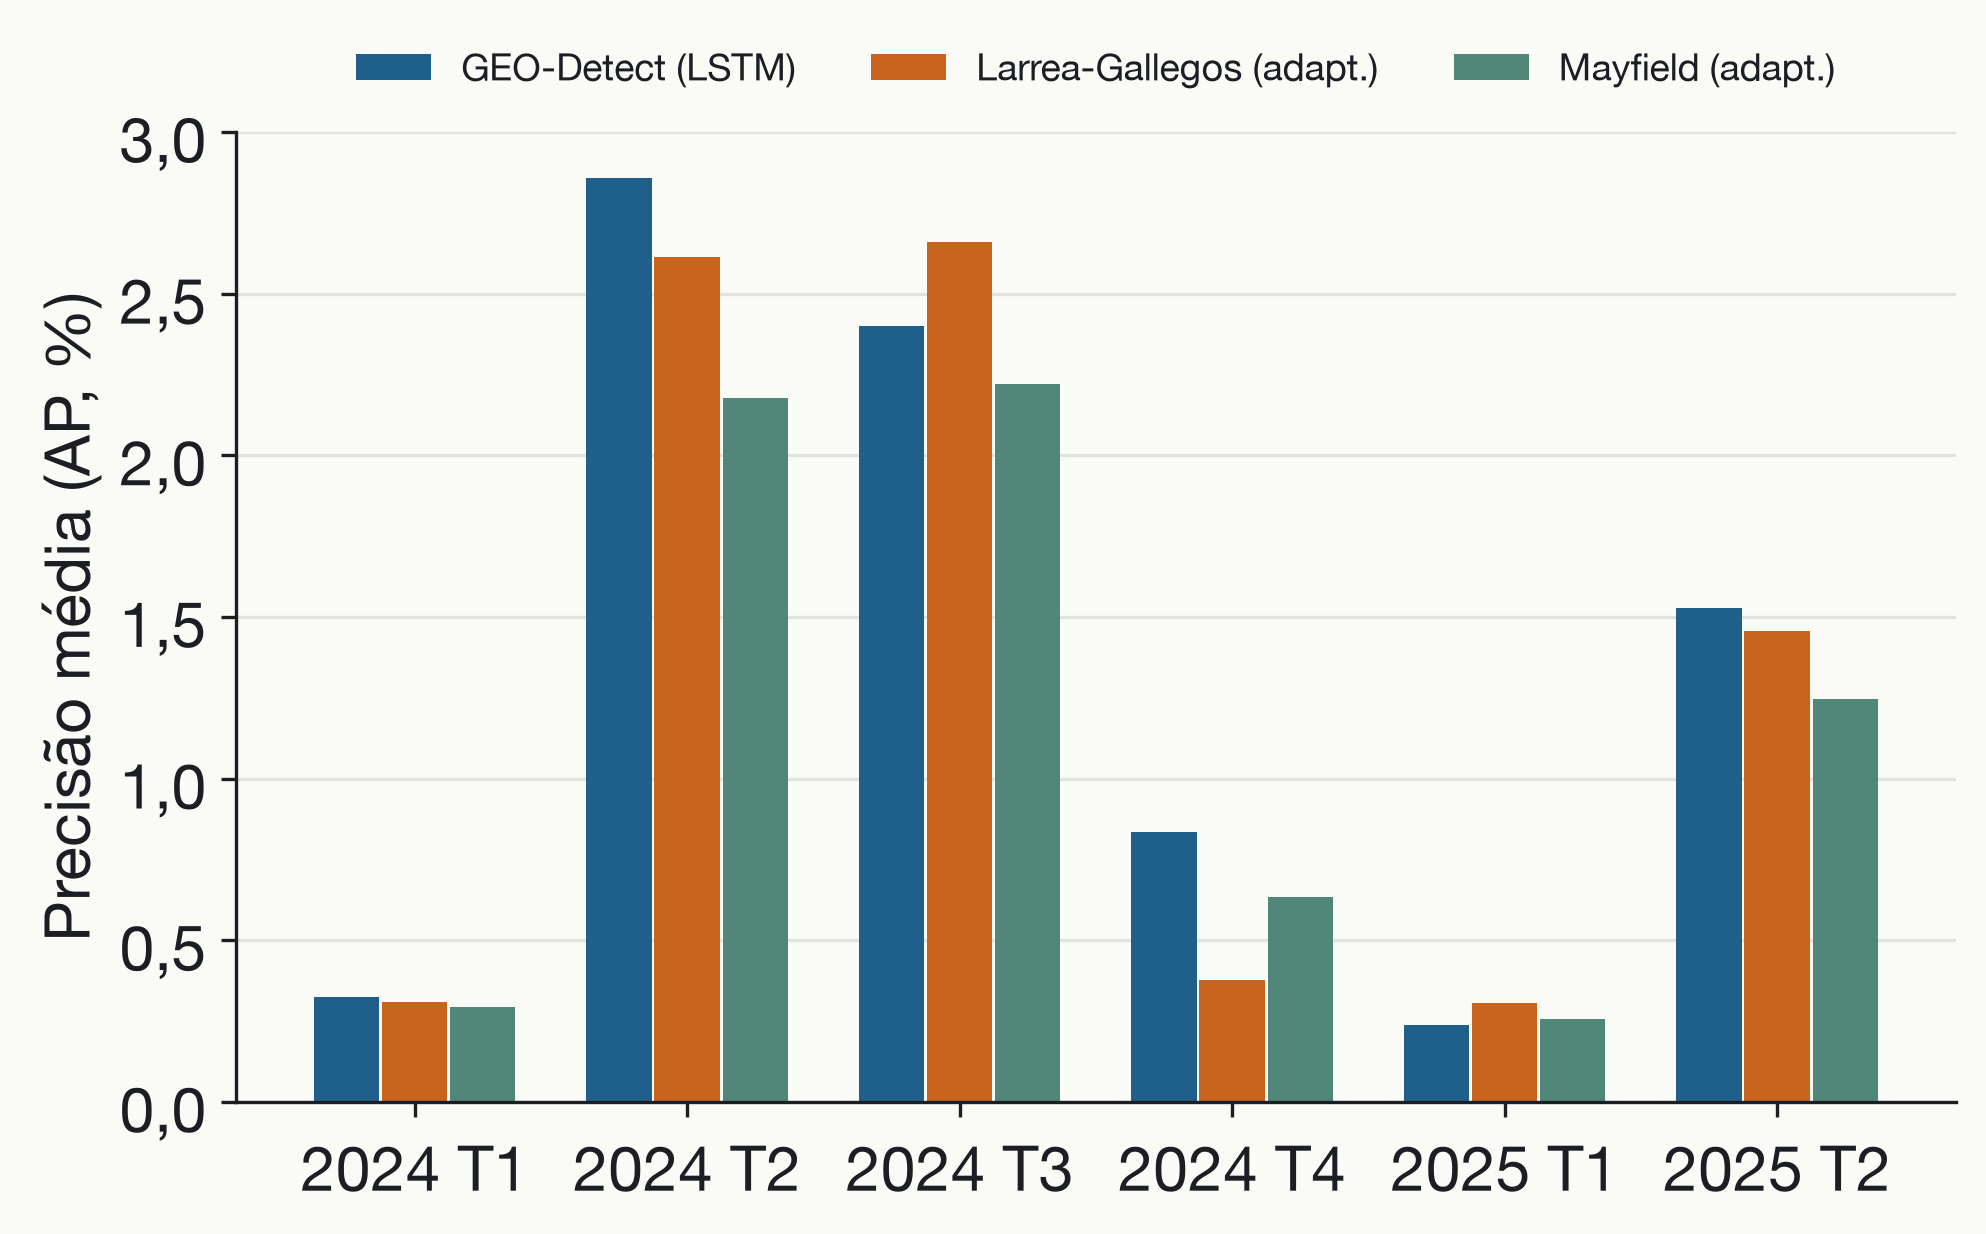
\includegraphics[width=\columnwidth]{../../results/poster/fig_precisao_alertas.png}
\caption{Precisão média por trimestre no Pará. Os valores das referências são de adaptações avaliadas neste estudo. Fonte: DETER/INPE, HydroRIVERS e IBGE.}
\label{fig:ap}
\end{figure}

Larrea-Gallegos et al. estudaram mineração aluvial na Amazônia peruana com Random Forest e variáveis de acessibilidade. Adaptamos a família do modelo para prever alertas trimestrais, com atributos históricos agregados e distâncias geográficas. Mayfield et al. avaliaram uma rede totalmente conectada de 60 unidades ocultas para desmatamento. A adaptação usa os mesmos preditores da LSTM, com a série mensal achatada.

Kanoga et al. fizeram previsão mensal de desmatamento em oito áreas da Amazônia brasileira, usando duas camadas LSTM e histórico DETER. O GEO-Detect adapta a arquitetura para mineração trimestral e acrescenta dados de hidrografia e localidades. Os artigos avaliam outros desfechos, recortes ou métricas. A comparação numérica da Fig.~\ref{fig:ap} tem como base as adaptações ao nosso protocolo.

\section{Conclusão}

O GEO-Detect avalia a previsão trimestral de alertas de mineração combinando séries temporais e dados geográficos. A precisão média foi baixa em termos absolutos. A análise no Pará é retrospectiva e usa trimestres já examinados no desenvolvimento. A generalização temporal exige novos períodos completos e uma configuração congelada.

\section{Materiais e rastreabilidade}

O pacote de reprodução inclui a extração congelada do DETER, o código, as versões das dependências e as 18 linhas de referência da comparação (três modelos por seis trimestres). O comando \texttt{python} \path{scripts/reproduzir_artigo.py}, executado a partir da raiz do pacote, obtém o HydroRIVERS e os arquivos do IBGE nos provedores oficiais. Ele verifica os hashes dos insumos, reexecuta os scripts 23 a 25 e confere as contagens e a AP de cada trimestre antes de gerar a Fig.~\ref{fig:ap}. O arquivo \path{reproducao/README.md} identifica o ambiente de referência e as saídas.

Código, dados de referência e instruções de reprodução no \href{https://github.com/HenriqueBuzin/GEO-Detect}{repositório GEO-Detect}.

\begin{thebibliography}{9}
\bibitem{hochreiter1997} S. Hochreiter and J. Schmidhuber, \emph{Long Short-Term Memory}. Neural Computation, v. 9, n. 8, p. 1735--1780, 1997. \href{https://doi.org/10.1162/neco.1997.9.8.1735}{DOI: 10.1162/neco.1997.9.8.1735}.

\bibitem{kanoga2024} S. Kanoga \emph{et al.}, \emph{A Recurrent Deep Learning-Based Monthly Deforestation Prediction Model in Eight Areas for Brazilian Amazon: A Pilot Study}. IGARSS 2024, 5208--5212. \href{https://doi.org/10.1109/IGARSS53475.2024.10642628}{DOI: 10.1109/IGARSS53475.2024.10642628}.

\bibitem{saito2015} T. Saito and M. Rehmsmeier, \emph{The Precision-Recall Plot Is More Informative than the ROC Plot When Evaluating Binary Classifiers on Imbalanced Datasets}. PLOS ONE, v. 10, n. 3, e0118432, 2015. \href{https://doi.org/10.1371/journal.pone.0118432}{DOI: 10.1371/journal.pone.0118432}.

\bibitem{sklearnap} SCIKIT-LEARN DEVELOPERS. \emph{average\_precision\_score}. Documentação da métrica. \href{https://scikit-learn.org/stable/modules/generated/sklearn.metrics.average_precision_score.html}{Disponível on-line}.

\bibitem{inpe} INSTITUTO NACIONAL DE PESQUISAS ESPACIAIS (INPE). \emph{DETER Amazônia}. Camada de avisos em áreas de floresta. \href{https://terrabrasilis.dpi.inpe.br/downloads/}{Disponível on-line}.

\bibitem{lehner2013} B. Lehner and G. Grill, \emph{Global river hydrography and network routing}. Hydrological Processes, 27(15), 2171--2186, 2013. Base HydroRIVERS v1.0. \href{https://doi.org/10.1002/hyp.9740}{DOI: 10.1002/hyp.9740}.

\bibitem{ibge} INSTITUTO BRASILEIRO DE GEOGRAFIA E ESTATÍSTICA (IBGE). \emph{Cadastro de localidades selecionadas}. Censo Demográfico 2010. \href{https://geoftp.ibge.gov.br/organizacao_do_territorio/estrutura_territorial/localidades/cadastro_de_localidades_selecionadas_2010/Shapefile_SHP/}{Disponível on-line}.

\bibitem{mayfield2020} H. J. Mayfield, C. Smith, M. Gallagher, and M. Hockings, \emph{Considerations for selecting a machine learning technique for predicting deforestation}. Environmental Modelling \& Software, 131, 104741, 2020. \href{https://doi.org/10.1016/j.envsoft.2020.104741}{DOI: 10.1016/j.envsoft.2020.104741}.

\bibitem{larrea2023} G. Larrea-Gallegos, R. Kahhat, I. Vázquez-Rowe, and E. Parodi, \emph{A machine learning approach to understand how accessibility influences alluvial gold mining expansion in the Peruvian Amazon}. Case Studies in Chemical and Environmental Engineering, 7, 100353, 2023. \href{https://doi.org/10.1016/j.cscee.2023.100353}{DOI: 10.1016/j.cscee.2023.100353}.

\end{thebibliography}
\end{document}
